\documentclass[11pt]{article}
\usepackage{geometry}                
\geometry{letterpaper}                   

\usepackage{graphicx}
\usepackage{amssymb}
\usepackage{epstopdf}
\usepackage{natbib}
\usepackage{amssymb, amsmath}

\usepackage[autolinebreaks,numbered]{mcode} % matlab code listings

\usepackage{natbib} % bibliography

\usepackage{pdfpages}

\DeclareGraphicsRule{.tif}{png}{.png}{`convert #1 `dirname #1`/`basename #1 .tif`.png}

%\title{Title}
%\author{Name 1, Name 2}
%\date{date} 

\begin{document}



\thispagestyle{empty}

\begin{center}
\includegraphics[width=5cm]{ETHlogo.eps}

\bigskip


\bigskip


\bigskip


\LARGE{ 	Lecture with Computer Exercises:\\ }
\LARGE{ Modelling and Simulating Social Systems with MATLAB\\}

\bigskip

\bigskip

\small{Project Report}\\

\bigskip

\bigskip

\bigskip

\bigskip


\begin{tabular}{|c|}
\hline
\\
\textbf{\LARGE{Stable Marriage Problem}}\\
\textbf{\LARGE{...}}\\
\\
\hline
\end{tabular}
\bigskip

\bigskip

\bigskip

\LARGE{Valentin Junet \& Samuel Imfeld}



\bigskip

\bigskip

\bigskip

\bigskip

\bigskip

\bigskip

\bigskip

\bigskip

Zurich\\
December 2014\\

\end{center}



\newpage

%%%%%%%%%%%%%%%%%%%%%%%%%%%%%%%%%%%%%%%%%%%%%%%%%

\newpage

\setcounter{page}{1}
\pagenumbering{roman}

\section*{Agreement for free-download}
\bigskip


\bigskip


\large We hereby agree to make our source code for this project freely available for download from the web pages of the SOMS chair. Furthermore, we assure that all source code is written by ourselves and is not violating any copyright restrictions.

\begin{center}

\bigskip


\bigskip


\begin{tabular}{@{}p{3.3cm}@{}p{6cm}@{}@{}p{6cm}@{}}
\begin{minipage}{3cm}

\end{minipage}
&
\begin{minipage}{6cm}
\vspace{2mm} \large Valentin Junet

 \vspace{\baselineskip}

\end{minipage}
&
\begin{minipage}{6cm}

\large Samuel Imfeld

\end{minipage}
\end{tabular}


\end{center}
\newpage

%%%%%%%%%%%%%%%%%%%%%%%%%%%%%%%%%%%%%%%

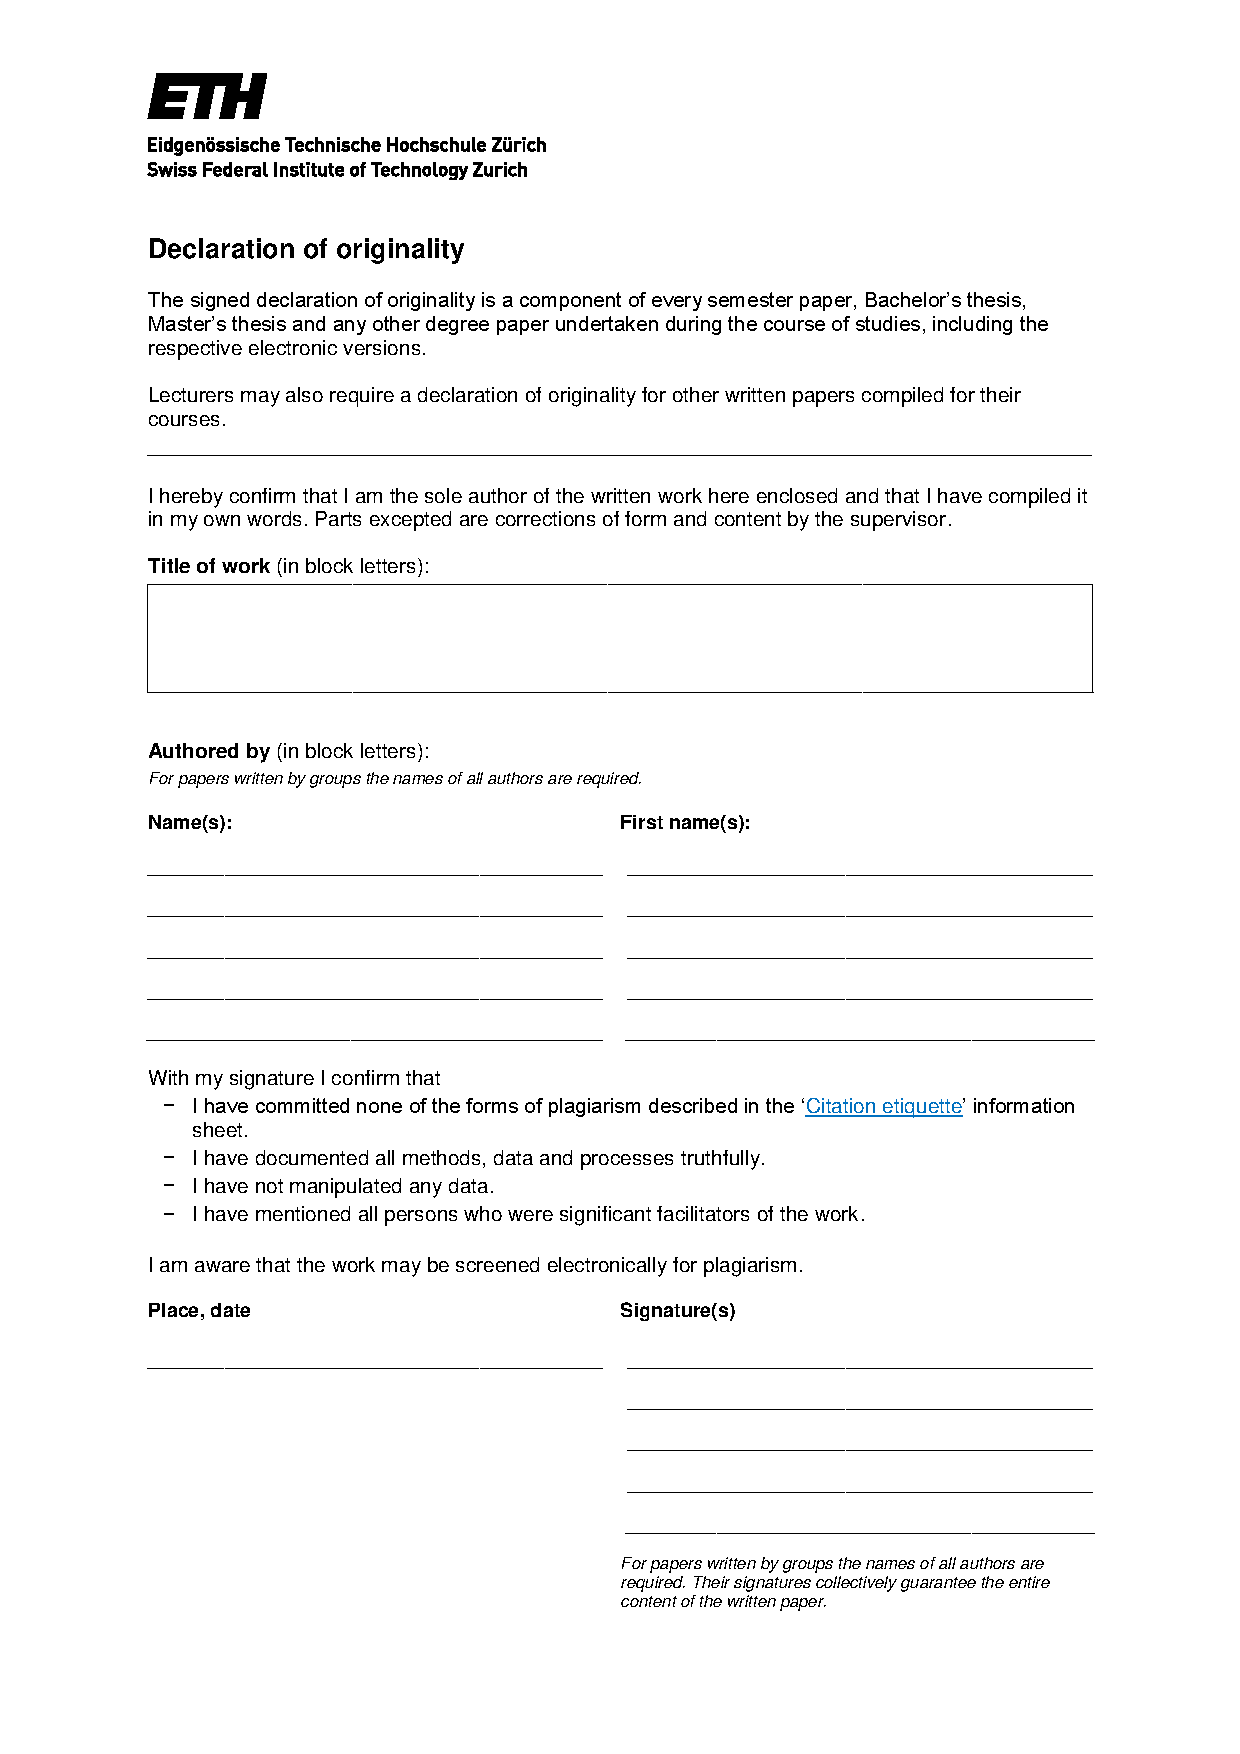
\includepdf{declaration-originality}

% IMPORTANT
% you MUST include the ETH declaration of originality here; it is available for download on the course website or at http://www.ethz.ch/faculty/exams/plagiarism/index_EN; it can be printed as pdf and should be filled out in handwriting


%%%%%%%%%% Table of content %%%%%%%%%%%%%%%%%

\newpage

\tableofcontents

\newpage

\setcounter{page}{1} % start page numbering here
\pagenumbering{arabic}

%%%%%%%%%%%%%%%%%%%%%%%%%%%%%%%%%%%%%%%



\section{Abstract}

\section{Individual contributions}

\section{Introduction and Motivations}

\section{Description of the Model}

\citet{1962} % test, to be removed

\section{Implementation}

\section{Simulation Results and Discussion}

\section{Summary and Outlook}

\section{References}

\bibliographystyle{plainnat}
\bibliography{references}

% jstor pdf link http://www.jstor.org/stable/pdfplus/2312726.pdf

\section{Appendix: MATLAB Codes}

\subsection*{generateRandom.m}
\lstinputlisting{../../code/generateRandom.m}
\subsection*{generatePlane.m}
\lstinputlisting{../../code/generatePlane.m}
\subsection*{vprintf.m}
\lstinputlisting{../../code/vprintf.m}
\subsection*{makeMatch.m}
\lstinputlisting{../../code/makeMatch.m}
\subsection*{checkEngagements.m}
\lstinputlisting{../../code/checkEngagements.m}
\subsection*{simulation.m}
\lstinputlisting{../../code/simulation.m}






\end{document}  



 
